\newpage
\justify
\chapter{Integraci\'on}

%\begin{figure}[h!]
%\begin{center}
%\includegraphics[scale=0.3]{Arq}
%\end{center}
%\caption{El m\'etodo exhaustivo para calcular el \'area de una circunferencia.}
%\end{figure}

\begin{center}
\begin{tcolorbox}[enhanced,colback=blue!5!white, colframe=blue!5!white, title=?`Qu\'e vas a aprender?,coltitle=black, attach boxed title to top center=
{yshift=-\tcboxedtitleheight/2},
boxed title style={size=small,colback=blue!50!white}]
\begin{enumerate}
\item A aplicar los conocimientos operativos necesarios para el c\'alculo de integrales de funciones polin\'omicas, racionales, algebraicas trascendentes de forma inmediata y por el m\'etodo de sustituci\'on.\\
\item A comprender la integral definida de una funci\'on, el teorema  fundamental  del c\'alculo y su aplicaci\'on en la determinaci\'on del \'area de una regi\'on definida por una funci\'on. 
\end{enumerate}
\end{tcolorbox}
\end{center}

\begin{center}
\begin{tcolorbox}[enhanced,colback=blue!5!white, colframe=blue!5!white, title=Resumen,coltitle=black, attach boxed title to top left=
{yshift=-\tcboxedtitleheight/2},
boxed title style={size=small,colback=blue!50!white}]
En este cap\'itulo se inicia el estudio de las integrales indefinidas y definidas. Sus definiciones formales, y los teoremas relevantes para su compresi\'on. Adem\'as, se presenta la t\'ecnica de integraci\'on por sustituci\'on como avance de lo que se desarrollar\'a en el segundo capitulo. 
\end{tcolorbox}
\end{center}
%\vspace{2cm}
%\setlength\columnsep{3cm}
%\setlength\columnwidth{10cm}
%\begin{multicols}{2}
\begin{tcolorbox}[enhanced,colback=blue!5!white, colframe=blue!5!white,title=Subtemas,coltitle=black, attach boxed title to top right=
{yshift=-\tcboxedtitleheight/2},
boxed title style={colback=blue!50!white}]%, sidebyside,righthand width=1cm
%\begin{multicols}{2}
\begin{enumerate}
\item[1.1] Integral indefinida
\item[1.2] Integraci\'on por sustutuci\'on 
\item[1.3] Funciones trigonom\'etricas inversas
\item[1.4] La notaci\'on sigma y sus propiedades 
%\columnbreak
\item[1.5] El problema del \'Area  
\item[1.6] Integral definida
\item[1.7] Teorema  fundamental del c\'alculo
\end{enumerate}
%\end{multicols} 
%\tcblower
%%%%%%%%%%%%%%%%%%%%%%%%%%%%%%%%%
\end{tcolorbox}
%%%%%%%%%%%%%%%%%%%%%%%%%%%%%% Mapa conceptual %%%%%%%%%%%%%%%%%%%%%%%%%%%%%%%%
\newpage
\thispagestyle{empty}

 \hfill \Large \textcolor{red!50!black}{Mapa Conceptual del Cápitulo.}\hfill\vspace{20pt}
 
\tikzset{
  block/.style={rectangle, draw, fill=blue!50!black, rounded corners, text centered,     text width = 10em, minimum height = 2em},text=white,font=\fontsize{14pt}{15pt}\selectfont,
  line/.style={draw, -latex',line width=2pt}
  }
\begin{figure}[H]
 \noindent\hspace*{-50pt}\scalebox{0.7}{
\begin{tikzpicture}[every node/.style={block},scale=1.5]
% Place nodes
% \node (optimization) {Given \\optimization problem};
% \node [right of=optimization, node distance=4cm]  (critical) {Find \\ critical points};
 \node [ node distance=4cm] (second) {Integrales};
\coordinate (case one) at (-5,0) ;
\coordinate (case two) at (5,0) ;
\coordinate (A1) at (-5,-1.7) ;
\coordinate (B1) at (5,-1.7) ;
\node[fill=fondpaille,draw=fondpaille,text=black, below =1cm of second](case three) {Se Clasifican};
\node[below = 3cm of case one](II){Integral \\Indefinida};
\node[below = 3cm of case two](ID){Integral Definida};
\node[fill=fondpaille,draw=fondpaille,text=black,below = 1.2cm of case three](more){Se conectan};
\node[below = 2cm of more](TF){Teorema Fundamental del Cálculo};
\node[fill=fondpaille,draw=fondpaille,text=black,below = 2cm of II](a){Definida por};
\node[fill=fondpaille,draw=fondpaille,text=black,below  = 2cm  of ID](b){Definida por};
\node[minimum height = 4.5em,text width = 30em,below = 3cm of a](min){$\displaystyle\int f(x)dx =F(x)+C \Longleftrightarrow F^{\prime}(x)=f(x)$};
\node[text width = 25em,below = 3cm of b](max){$\displaystyle\lim_{n\rightarrow \infty}\sum_{i=1}   ^{n}f(x_i)\Delta x = \displaystyle\int_{a}^{b} f(x)dx  $};
\node[text width = 2em,fill=fondpaille,draw=fondpaille,text=black,below = 2cm of min](SI){Si};
\node[fill=fondpaille,draw=fondpaille,text=black,below = 2cm of max](AP){Aplicación};
\node[below = 2cm of SI](IT){$f(x)=\frac{1}{\sqrt{a^2-x^{2}}}
       $\\
       $f(x)=\frac{1}{x\sqrt{x^{2}-a^2}}$\\
       $f(x)=\frac{1}{x^{2}+a^2 }$};
\node[text width = 6em,fill=fondpaille,draw=fondpaille,text=black,below = 3.5cm of IT](C){Conduce};
\node[right = 2.5cm of C](FTI){Funciones Trigonométricas Inversas};
\node[text width = 12em,right = 3cm of SI](DEF){$f(x)=h(g(x))g^{\prime}(x)$};
\node[fill=fondpaille,draw=fondpaille,text=black,below = 2cm of DEF](U){Utilizamos};
\node[below = 2cm of U](MS){Método de Sustitución};
\node[below = 2cm of AP](ADC){Determinar el Área Debajo de la Curva, si $f(x)\geq0$};
% Draw edges
\draw [line] (second) -- (case three);
\draw [line,-] (case three) -- (A1);
\draw [line,-] (case three) -- (B1);
\draw [line] (A1) -- (II);
\draw [line] (B1) -- (ID);
\draw [line] (more) -- (II);
\draw [line] (more) -- (ID);
\draw [line] (more) -- (TF);
\draw [line] (II) -- (a);
\draw [line] (ID) -- (b);
\draw [line] (a) -- (min);
\draw [line] (b) -- (max);
\draw [line] (min) -- (SI);
\draw [line] (SI) -- (IT);
\draw [line] (SI) -- (DEF);
\draw [line] (DEF) -- (U);
\draw [line] (U) -- (MS);
\draw [line] (max) -- (AP);
\draw [line] (AP) -- (ADC);
\draw [line] (IT) -- (C);
\draw [line] (C) -- (FTI);
\end{tikzpicture}
                  }
  \end{figure}
\newpage
%%%%%%%%%%%%%%%%%%%%%%%%%%%%%% Mapa Mental %%%%%%%%%%%%%%%%%%%%%%%%%%%%%%%%%%%%
%\begin{tcolorbox}[colback=blue!5!white, colframe=blue!5!white] 
%¿Qu\'e vas a apender?
%\end{tcolorbox}
%\end{multicols}
\thispagestyle{empty}
%\begin{landscape} % cargar paquete pdflscape
%\thispagestyle{empty}
%\psset{unit=1.1}
%%\hspace*{3cm}
%\begin{pspicture}(0,-5)(15,5)
%%\malla
%\rput(3,6.7){\textcolor{red!50!black}{ \bf \Large  Mapa conceptual del cap\'itulo I:}}
%\rput(7,6){\psframebox{\large Integrales}}
%\rput(7,5){\rnode{a1}{se clasifican en}}
%\qline(7,5.8)(7,5.2)
%%% Izquierdo
%%%-----------------------------------
%\qline(5,5)(0,5)
%\psline{->}(0,5)(0,4.5)
%\rput(0,4){\rnode{a2}{\psframebox{Integral indefinida}}} 
%\psline{->}(0,3.7)(0,3.1)
%\rput(0,2.9){\rnode{b1}{definida por}}
%\psline{->}(0,2.7)(0,2)
%\rput(1,1.5){\rnode{a3}{ \psframebox{$\displaystyle\int f(x)dx =F(x)+C \Longleftrightarrow F^{\prime}(x)=f(x)$}}}
%\psline{->}(0,1)(0,0.5)
%\rput(0,0.2){si}
%\psline{->}(0,-0.1)(0,-0.5)
%\psline{->}(0.5,0.2)(3,0.2)
%\rput(5,0){\rnode{a5}{\psframebox{$f(x)=h(g(x))g^{\prime}(x)$}}}
%\psline{->}(5,-0.5)(5,-1)
%\rput(5,-1.3){utilizamos}
%\psline{->}(5,-1.5)(5,-2)
%\rput(5,-2.5){\rnode{a4}{\psframebox{M\'etodo de sustituci\'on}}}
%\rput(0.2,-1){$f(x)=\frac{1}{\sqrt{a^2-x^{2}}}
% $}
%\rput(0.2,-2){$f(x)=\frac{1}{x\sqrt{x^{2}-a^2}}$}
%\rput(0.2,-3){$f(x)=\frac{1}{x^{2}+a^2 }$}
%\psframe(1.5,-0.5)(-1,-3.5)
%\psline{->}(0,-3.5)(0,-4.4)
%\rput(0,-4.5){conduce a}
%\psline{->}(1,-4.5)(2.8,-4.5)| 
%\rput(5,-4.5){\psframebox{F. trigonom\'etricas inversa }}
%%% Derecho F. trigonom\'etricas inversa
%%%-----------------------------------
%\qline(9,5)(14,5)
%\psline{->}(14,5)(14,4.5)
%\rput(14,4){\rnode{a7}{\psframebox{Integral definida}}} 
%\psline{->}(14,3.5)(14,3)
%\rput(14,2.5){definida por}
%\psline{->}(14,2.3)(14,1.6)
%\rput(14,1){\rnode{a8}{\psframebox{ $\displaystyle\lim_{n\rightarrow \infty}\sum_{i=1}^{n}f(x_i)\Delta x = \displaystyle\int_{a}^{b} f(x)dx  $}}}
%\psline{-}(14,0)(14,-1)
%\psline{->}(14,-1)(13,-1)
%\psline{->}(12.5,4)(9,4)
%\psline{->}(2,4)(6,4)
%\psline{->}(7.5,3.5)(7.5,2.3)
%%\psline{->}(7,2)(5.5,2)
%\rput(7.5,4){se conectan en}
%\rput(7.5,2){\rnode{a9}{\psframebox{Teorema fundamental}}} 
%%\rput(5,2){SI}
%%\psline{->}(5,1.8)(5,0.8)
%\rput(12,-1){\rnode{a9}{Aplicaci\'on}}
%\psline{->}(12,-1.5)(12,-2.5)
%\rput(12,-3){\psframebox{Determinar el \'area bajo la curva, si $f\geq 0$}} 
%\end{pspicture}
%\end{landscape} 
 %%%%%%%%%%%%%%%%%%%%%%%%%%%%%%%%%%%%%%%%%%%%%%%%%%%%%%%%%%%%%%%%%%%%%%%%%%%%%%
 \hfill\Large \textcolor{red!50!black}{Mapa Mental del Cápitulo.}\hfill\vspace{20pt}

\begin{figure}[H]
\centering
  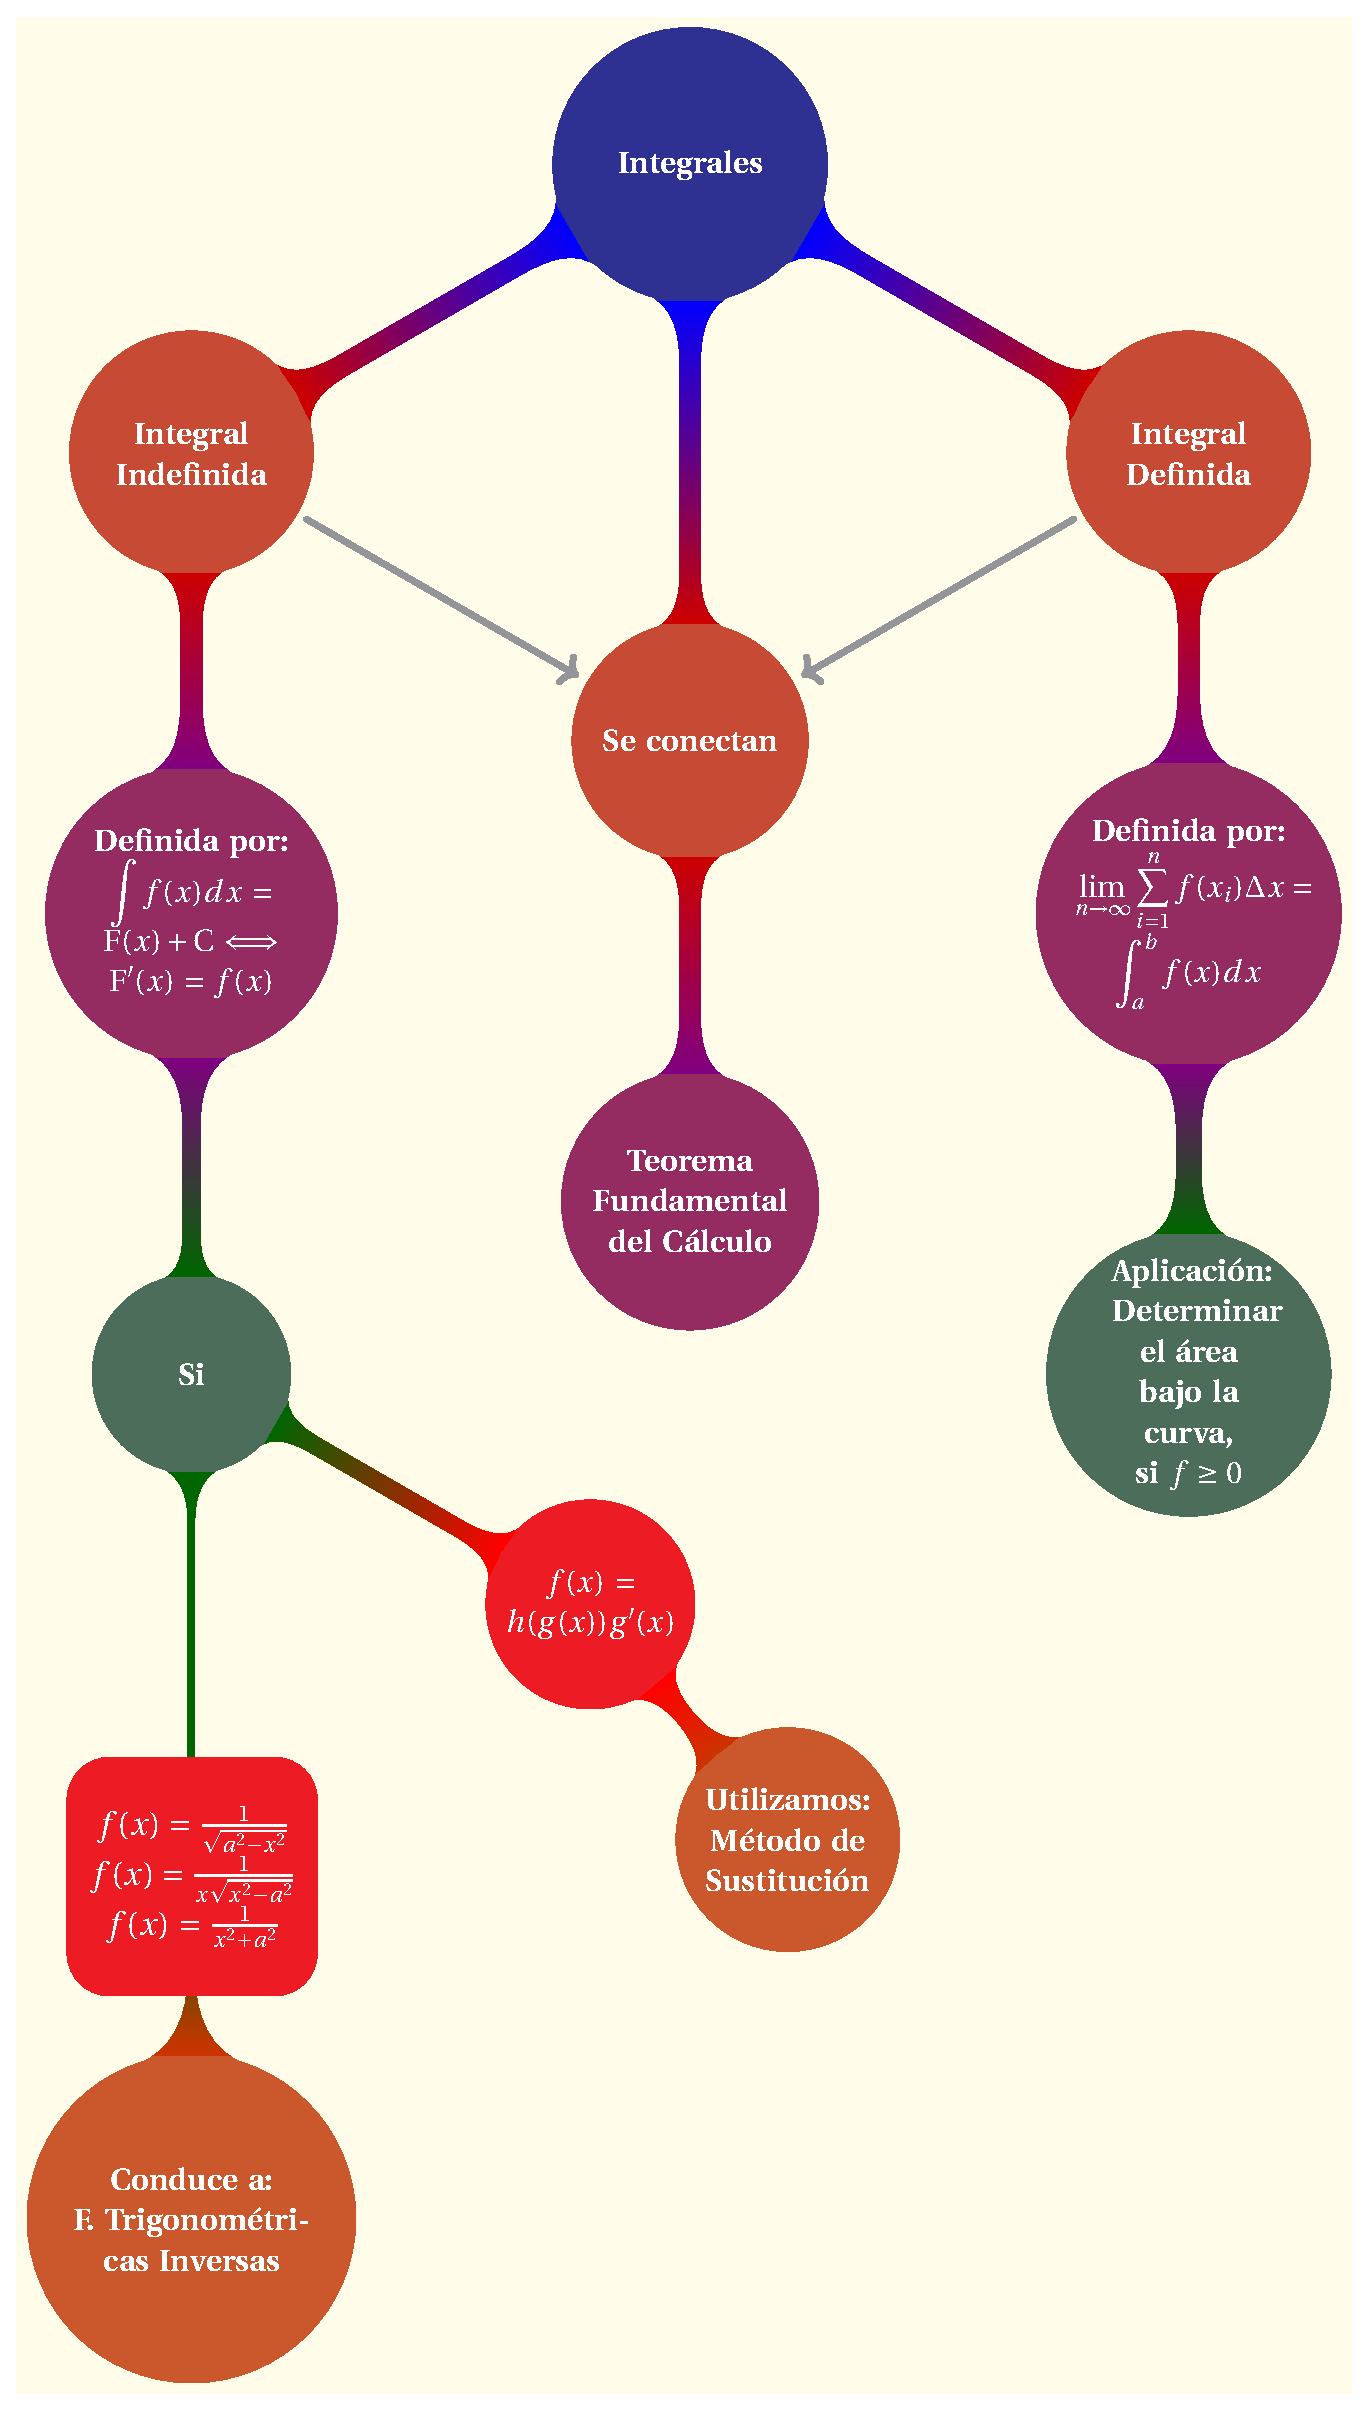
\includegraphics[scale=0.5]{pdf/mindmap-integrales-escale} 
 \end{figure}
\newpage
 

\section{Integral indefinida}


En el curso de c\'alculo diferencial hemos estudiado el procedimiento para a partir de una funci\'on $F$ determinar su derivada, la cual denotaremos como $f$. Sin embargo, existen situaciones en donde conocemos la derivada $f$ y pretendemos obtener la funci\'on $F$. En ese caso, $F$ se conoce como la antiderivada. A continuaci\'on presentaremos el concepto de antiderivada o primitiva y f\'ormulas b\'asicas para determinarla . \vspace*{0.3cm}

\begin{definicion}{Antiderivada}{FA}\label{def-funcion-F}
Una funci\'on $F:I \to \mathbb R$ es una \textbf{antiderivada}  o primitiva para una funci\'on  $f:I \to \mathbb R$ en el intervalo $I$, si $$F^{\prime}(x)= f(x)$$  para todo $x\in I$. Si $x$ es punto extremo del intervalo $I,$ la derivada es la derivada lateral respectiva.
\end{definicion}
\vspace*{0.2cm}
\marginpar{\begin{observacion}{}{}
En la practica generalmente no hacemos menci\'on del intervalo $I,$ mas la primitiva de una funci\'on siempre ser\'a definida en un intervalo.
\end{observacion}}

%%%%%%%%%%%%%%%%%%%%%%%%%%%%%%%%%%%%%%%%%%%%%
\begin{Ejemplo}\label{ej1}
Sea $$P(x)=\frac{1}{4} x^{4}-3\sqrt{x}+\frac{1}{x^2}.$$ Muestre que $P$ es antiderivada de $p(x)=x^3-\frac{3}{2\sqrt{x}}-\frac{2}{x^3}$.
\end{Ejemplo}

\begin{proof}
Derivando la funci\'on $P$, obtenemos
$$P^{\prime}(x)=x^3-\frac{3}{2\sqrt{x}}-\frac{2}{x^3}=p(x)$$ 
\end{proof}


%%%%%%%%%%%%%%%%%%%%%%%%%%%%%%%%%%%%%%%%%%%

\noindent Con relaci\'on al ejemplo anterior, se puede observar que $P$ no es la \'unica antiderivada de $p$, puesto que $F(x)=\frac{1}{4} x^{4}-3\sqrt{x}+\frac{1}{x^2}+C$, $C\in\R$,  es tambie\'n una antiderivada de $p$. El siguiente resultado muestra que si se conoce una antiderivada  de una funci\'on entonces se puede encontrar otra antiderivada agregando una constante arbitraria.   

\begin{proposicion}{}{TeoAnt}\label{teo-antiderivada-G}
Sea $F:I \to \mathbb R$ una primitiva para la funci\'on  $f:I \to \mathbb R$ en el intervalo $I.$ Entonces
$$G(x):=F(x)+C, \quad C\in\mathbb R,$$ es tambi\'en una primitiva de $f$ en $I.$
\end{proposicion}

\begin{Ejemplo}\label{ej2} Dada la funci\'on:
\begin{align*}
 f(x)= \frac{\sen^{2}(x)+\cos^{4}(x)+\sen^{2}(x)\cos^{2}(x)}{\cos^{2}(x)}.
\end{align*}
Pruebe que $F(x)=\tan(x)+C$, $C\in\R$, es antiderivada de $f(x).$
 \end{Ejemplo}
\begin{proof} 
Observe que $F^{\prime}(x)=\sec^{2}(x)$. Al simplificar la funci\'on  $f$, tenemos que
\begin{align*}
f(x)&= \frac{\sen^{2}(x)+\cos^{4}(x)+\sen^{2}(x)\cos^{2}(x)}{\cos^{2}(x)}\\
&=\frac{\sen^{2}(x)}{\cos^{2}(x)}+\frac{\cos^{4}(x)}{\cos^{2}(x)}+\frac{\sen^{2}(x)\cos^{2}(x)}{\cos^{2}(x)} \\
&=\tan^{2}(x)+\cos^{2}(x)+\sen^{2}(x) \\
&=\tan^{2}(x)+1 \\
&=\sec^{2}(x).
\end{align*}
De donde se concluye que $F(x)=\tan(x)+C$ es antiderivada de $f(x)$. 
\end{proof}\\

 
Una pregunta natural que surge, es la siguiente: si $F$ y $G$ son primitivas de una funci\'on $f$ en un intervalo $I,$ 
\begin{center}
?`ser\'a que $F$ y $G$ est\'an relacionadas de alguna manera? 
\end{center}
La respuesta a este interrogante est\'a dada por el siguiente resultado.
 
%\psset{unit=0.8}
\marginpar{
%\scalebox{0.5}{
% \begin{pspicture}(-4,-4)(4,4)
%%\malla
%\psaxes{<->}(0,0)(-4,-4)(4,4)  \psset{algebraic,plotpoints=501} 
%\psplot[linecolor=Turquoise!55!black ,linewidth=5\pslinewidth]{-2}{2}{x^2}
%\psplot[linecolor=Turquoise!55!black ,linewidth=5\pslinewidth]{-2}{2}{x^2-2}
%\psplot[linecolor=Turquoise!55!black ,linewidth=5\pslinewidth]{-2}{2}{x^2-4}
%\rput(2.5,-3){\textcolor{Turquoise!55!black}{C=-4}}
%\rput(2.5,1){\textcolor{Turquoise!55!black}{C=-2}}
%\rput(2.5,3){\textcolor{Turquoise!55!black}{C=0}}
%\rput(0,-4.5){$\Huge \displaystyle\int 2x \ dx = x^2 + C
%$}
%%\psplot[linecolor=red,linewidth=5\pslinewidth]{-2.5}{2.5}{x^2+2}
%%\psplot[linecolor=red,linewidth=5\pslinewidth]{-2.5}{2.5}{x^2-2}
%\end{pspicture}}
\begin{tikzpicture} [scale=0.5,font=\fontsize{7pt}{8pt}\selectfont]
     \tkzInit[xmin = -3, xmax = 4.5,ymin = -5, ymax =4]
     %\tkzDrawXY
%\tkzGrid[color=gray!40,line width=0.2pt]
\tkzDrawX[color=black,label={$x$},above left=5pt]
\tkzLabelX[color=black,orig=false]
\tkzDrawY[color=black,label={$y$},below right=5pt]
\tkzLabelY[color=black,orig=false]
     \tkzFct[domain = -2:2,blue,ultra thick]{x**2} 
     \tkzFct[domain = -2:2,blue,ultra thick]{x**2-2} 
     \tkzFct[domain = -2:2,blue,ultra thick]{x**2-4} 
 \tkzText[draw=red,fill = red!20,font=\fontsize{8pt}{9pt}\selectfont](0.1,5.7){$\displaystyle\int 2x \ dx = x^2 + C
$}  
 \tkzText[draw=red,fill = red!20,font=\fontsize{4pt}{5pt}\selectfont](2.9,4.2){$C=0$}  
\tkzText[draw=red,fill = red!20,font=\fontsize{4pt}{5pt}\selectfont](3,2.2){$C=-2$} 
\tkzText[draw=red,fill = red!20,font=\fontsize{4pt}{5pt}\selectfont](3,0.3){$C=-4$} 
      \end{tikzpicture}
                                         }

\begin{proposicion}{}{TeoAnt}\label{teo-antiderivada-G}
Si $F, G:I \to \mathbb R$ son primitivas de una funci\'on $f:I \to \mathbb R$ en el intervalo $I,$ entonces existe  $C\in\mathbb R$ tal que
$$G(x)=F(x)+C,$$ para todo $x\in I.$
\end{proposicion}
\vspace*{0.5cm}

A continuaci\'on vamos a presentar el concepto de integral indefinida. \\
 
\begin{definicion}{}{Integral Indefinida}
 Sea $F:I \to \mathbb R$ una primitiva para la funci\'on $f:I \to \mathbb R$ en el intervalo $I.$ La expresi\'on $$ F(x)+C, \quad C\in\mathbb R$$ es llamada la \textbf{integral indefinida} de la funci\'on $f$ y es denotada por 
\begin{align}\label{II}
\displaystyle\int f(x)\,dx=F(x)+C.
\end{align}
Es decir, $$\displaystyle\int f(x)\,dx=F(x)+C \Longleftrightarrow F^{\prime}(x)=f(x), \quad x\in I.$$
En \eqref{II} $f(x)$ es llamada integrando y $dx$ es el diferencial de $x$. 
\end{definicion}
\vspace*{0.5cm}

\begin{Ejemplo} Con relaci\'on a los Ejemplos \ref{ej1} y \ref{ej2} tenemos que, 
\begin{align*}  
  \displaystyle\int \left( x^3-\frac{3}{2\sqrt{x}}-\frac{2}{x^3} \right) \ dx &= \frac{1}{4} x^{4}-3\sqrt{x}+\frac{1}{x^2} + C \\
   \displaystyle\int \sec^{2}(x) \ dx &= \tan(x)+C
\end{align*} 
\end{Ejemplo}

Para nuestro prop\'osito inmediato, el diferencial $dx$ nos indica la variable de integraci\'on. Sin embargo, m\'as adelante y en especial en el Cap\'itulo 2 se expone m\'as sobre su importancia. Por otro lado, aunque la mayor\'ia de las funciones que aparecen com\'unmente poseen antederivada o primitiva, se debe preguntar que condiciones son necesarias para su existencia.  \\


\noindent \textcolor{red!50!black}{\LARGE \bf  Reglas b\'asicas de integraci\'on}   \vspace*{10pt} \\
% {\sc  }\label{rbi}
\noindent
A partir de las propiedades de la diferenciaci\'on se pueden obtener la antiderivada de algunas funciones de forma inmediata. En cada caso se tiene en cuenta la constante de integraci\'on. Por ejemplo
\begin{align*}
\frac{d}{dx}[\tan (x)]=\sec^{2}(x) \qquad entonces \quad \int \sec^{2}(x) \  dx= \tan (x) +C  \quad C\in \R
\end{align*}

%\newpage

\textbf{Integrales algebraicas:}
\begin{table}[h]
\begin{tcolorbox}[boxrule=0.2pt, enhanced,sharp corners, width=12cm,colframe=blue!8!black,colback=blue!5!white,drop lifted shadow=blue ]
\begin{multicols}{2}
\begin{list}{}{}
\item Derivadas
\item  $\dfrac{d}{dx}[kx] = k$
\item   $\dfrac{d}{dx}[x^{n}] = nx^{n-1}$
\columnbreak
\item Integrales
\item   $\displaystyle \int k\,dx=kx+C$
\item   $\displaystyle \int x^n\,dx=\frac{x^{n+1}}{n+1}+C,$ 
 \end{list}
 \end{multicols}
\hspace*{6.5cm} Con  $n\neq-1$
\end{tcolorbox}
\end{table}

 

\begin{Ejemplo} Determine las siguientes integrales
\begin{multicols}{2}
\begin{enumerate}
\item $\displaystyle\int  x^{2}\,dx $
\item $\displaystyle\int \sqrt{x}\,dx$
\columnbreak
\item $\displaystyle\int x^{-1/3}\,dx$
\item $\displaystyle\int \frac{dx}{x^3}$
\end{enumerate}
\end{multicols}
\end{Ejemplo}

\begin{proof}
\begin{enumerate}
\item $\displaystyle\int  x^{2} \,dx =   \displaystyle\int x^{2} \,dx  = \frac{ x^3}{3}+C$ \\
\item  $\displaystyle\int \sqrt{x}\,dx =\displaystyle\int x^{1/2}\,dx = \frac{2}{3} x^{3/2} +C $ \\
\item   $\displaystyle\int x^{-1/3}\,dx= \frac{x^{2/3} }{2/3} +C = \frac{3}{2} x^{2/3}  +C $\\
\item $\displaystyle\int \frac{dx}{x^3}  = \displaystyle\int x^{-3}\,dx =  -\frac{x^{-2} }{2} +C = -\frac{1}{2x^2} +C  $  
%  \item $\displaystyle\int \frac{1}{x^4}\,dx$
\end{enumerate}
\end{proof}


\begin{teorema}{Linealidad de la integral}{}
Sean $F, G:I \to \mathbb R$  primitivas de  $f, g:I \to \mathbb R$ respectivamente, en el intervalo $I,$ y $\beta\in \mathbb R.$ Entonces $F+\beta G$ es una primitiva para $f+ \beta g$ en $I,$ y $$ \int [f(x)\pm \beta g(x)]dx= \int f(x)dx\pm \beta \int g(x)dx $$
\end{teorema}

%\textbf{Linealidad de la integral:}
%\begin{table}[h]
%\begin{tcolorbox}[boxrule=0.2pt, enhanced,sharp corners,   width=12cm,colframe=blue!8!black,colback=blue!5!white,drop lifted shadow=blue ]

%\begin{enumerate}
   %\item ${\tiny \displaystyle \int [f(x)\pm g(x)]dx= \int f(x)dx\pm\int g(x)dx}$
 %\item $\displaystyle \int k f(x)\,dx=k\int f(x)\,dx$
  %\item $\displaystyle \int g(x)f(x)\,dx \neq \int g(x)\,dx\int f(x)\,dx$
% \end{enumerate}
%\end{tcolorbox}
%\end{table}


\begin{Ejemplo} Determine las siguientes integrales indefinidas
\begin{multicols}{2}
\begin{enumerate}
\item $\displaystyle\int (3x^3-5x^2)\,dx$
\item $\displaystyle\int \frac{x+1}{\sqrt{x}}\,dx$
\item $\displaystyle\int (\sqrt{x}+1)(x-\sqrt{x}+1)dx$
\columnbreak
%\item $\displaystyle\int (a+bx^3)^2 \ dx$
\item $\displaystyle\int  z(z+a)(z+b) \ dz $
\item $\displaystyle\int \dfrac{(x^2+1)(x^2-2)}{x^{2/3}}\,dx$
\item $\displaystyle\int \dfrac{(x^m-x^n)^2}{\sqrt{x}}dx$
\end{enumerate}
\end{multicols}
\end{Ejemplo}

\begin{proof}
\begin{enumerate}
\item  $\displaystyle\int (3x^3-5x^2)\,dx = 3\displaystyle\int x^3 \,dx -5\displaystyle\int x^2\,dx = \frac{3}{4}x^4-\frac{5}{3}x^3+C$ \\
\item $\displaystyle\int \frac{x+1}{\sqrt{x}}\,dx  =\displaystyle\int \left( \frac{x}{\sqrt{x}}+\frac{1}{\sqrt{x}}\right) \,dx = \frac{2}{3}x^{3/2}+2x^{1/2}+C
$ \\
\item $\displaystyle\int (\sqrt{x}+1)(x-\sqrt{x}+1)dx  =\displaystyle\int( x^{3/2}+1)dx  = \frac{2}{5}x^{5/2}+x+C $ \\
% \item $\displaystyle\int (a+bx^3)^2 \ dx=  \displaystyle\int (a^2 + 2abx^3 + b^2x^6) \ dx=\frac{a^3}{3}+\frac{1}{2}abx^4+\frac{b^2}{7}x^7+C$ \\
\item   $\begin{aligned}[t]
\displaystyle\int  z(z+a)(z+b) \ dz &=\displaystyle\int   (z^2+az)(z+b) \ dz =\displaystyle\int   (z^3 +bz^2 +az^2+abz) \ dz \\
  &=\displaystyle\int   (z^3 +(b+a)z^2+abz) \ dz =\frac{z^4}{4}+\frac{(b+a)}{3}z^{3}+\frac{ab}{2}z^2+C
 \end{aligned}$ \\
\item $\begin{aligned}[t] \displaystyle\int \dfrac{(x^2+1)(x^2-2)}{x^{2/3}} dx &= \displaystyle\int \dfrac{x^4 -x^2-2}{x^{2/3}}dx =\displaystyle\int \left(\dfrac{x^4}{x^{2/3}}  -\dfrac{x^2}{x^{2/3}}  -\dfrac{2}{x^{2/3}} \right)dx \\
 &= \displaystyle\int \left( x^{10/3}  -x^{4/3}  - 2x^{-2/3} \right)dx  =\frac{3}{13}x^{13/3} -\frac{3}{7}x^{7/3}-4x^{1/2}+C \end{aligned}$
 \item Supongamos que $n \neq m$ y $n,m \neq 0$
\begin{align*}
 \displaystyle\int \dfrac{(x^m  -x^n)^2}{\sqrt{x}}\,dx &=\displaystyle\int \dfrac{ x^{2m}-2x^{m+n}+x^{2n} }{\sqrt{x}}\,dx \\
 &  =\displaystyle\int  \left( x^{2m-1/2}-2x^{m+n-1/2}+x^{2n-1/2} \right) \,dx \\
 &=\sqrt{x}\left( \frac{2x^{2m}}{4m+1}-\frac{2x^{m+n}}{2m+2n+1}+\frac{2x^{2n}}{ 4n+1  }\right)+C
\end{align*} 
\end{enumerate}
\end{proof}
%&=\frac{x^{2m+1/2}}{2m+1/2}-\frac{2x^{m+n+1/2}}{m+n+1/2}+\frac{x^{2n+1/2}}{2n+1/2}+C  \\
% & =\frac{2x^{(4m+1)/2}}{ 4m+1  }-\frac{4x^{(2m+2n+1) }}{2m+2n+1}+\frac{2x^{(4n+1)/2}}{ 4n+1  }+C
%& = \frac{x^{(4m+1)/2}}{(4m+1)/2}-\frac{2x^{(2m+2n+1)/2}}{(2m+2n+1)/2}+\frac{x^{(4n+1)/2}}{(4n+1)/2}+C
% %\\  \\
\\
\newpage

\textbf{Trigonom\'etricos:}

\begin{table}[h]
\begin{tcolorbox}[boxrule=0.2pt, enhanced,sharp corners,   width=14cm,colframe=blue!8!black,colback=blue!5!white,drop lifted shadow=blue ]
\begin{footnotesize}
\begin{multicols}{2}
\begin{list}{}{}
\item Derivadas
\item $\dfrac{d}{dx}[\cos(x)]=-\sin(x) $
\item $\dfrac{d}{dx}[\sin(x)]=\cos(x)$
\item $\dfrac{d}{dx}[\tan(x)]= \sec^{2}(x)$
\item $\dfrac{d}{dx}[\cot(x)]= -\csc^{2}(x)$
\item $\dfrac{d}{dx}[\sec(x)]= \sec(x)\tan(x)$
\item $\dfrac{d}{dx}[\csc(x)]= -\csc(x)\cot(x)$
\columnbreak
\item Integrales
\item $\displaystyle \int \sin(x)\,dx=-\cos(x)+C$
\item $\displaystyle \int \cos(x)\,dx=\sin(x)+C$
\item $\displaystyle \int \sec^{2}(x)\,dx=\tan(x)+C$
\item $\displaystyle \int \csc^{2}(x)\,dx=-\cot(x)+C$
\item $\displaystyle \int \sec(x)\tan(x)\,dx=\sec(x)+C$
\item $  \displaystyle \int \csc(x)\cot(x)\,dx=-\csc(x)+C$
\end{list} 
\end{multicols}
\end{footnotesize}
\end{tcolorbox}
\end{table}


\begin{Ejemplo} Determine las siguientes integrales indefinidas
\begin{multicols}{2}
\begin{enumerate}
%\item $\displaystyle\int 2\sin(x)\,dx$
\item  $ \displaystyle\int\dfrac{2\cot\; x - 3 \sen^2 x}{\sen x}dx$
%\item $\displaystyle\int \sqrt{1-\cos^{2} (x)} \  dx$ \\
\columnbreak
\item  $ \displaystyle\int\dfrac{4\csc^2 t \ \cos t- \tan t }{\cos t}dt$
%\item $\displaystyle\int  \cot^{2} (t),dt$ \\
\end{enumerate}
\end{multicols}
\end{Ejemplo}


\begin{proof}
\begin{enumerate}
 % \item  $\displaystyle\int 2\sin(x)\,dx= 2\displaystyle\int \sin(x)\,dx = 2 cos(x)+C$ \\
 \item  Recuerde que $\csc (x)=\dfrac{1}{\sen (x)}$.
\begin{align*}
  \ \int\frac{2\cot\; (x) - 3 \sen^2 (x)}{\sen (x)}dx &= 2\int\frac{1}{\sen (x)} \cot (x)  dx -3 \int\sen (x) dx \\
   & = -2\csc\;(x)+3 \cos\; (x)+C.
\end{align*}%&= 2\int\csc\; (x) \cot\; (x) dx-3\int\sen\; (x) dx  \\
%\item Recuerde que $\sin^2(x)+\cos^2(x)=1$
%\begin{align*}
%  \displaystyle\int \sqrt{1-\cos^{2} (x)} \  dx &= \displaystyle \int \sqrt{\sin^2(x)} \  dx \\
%  &= \displaystyle \int  \sin(x) \  dx = -\cos(x)+C
%\end{align*}
\item Recuerde que  $\sec (t)=\dfrac{1}{\cos (t)}$
\begin{align*}
 \displaystyle\int\dfrac{4\csc^2 (t) \ \cos (t)- \tan (t) }{\cos (t)}dt &= 4\int \csc^2 (t)\,dt - \int \frac{\tan (t)}{\cos (t) } dt\\
   &= 4\int \csc^2 (t) - \int \sec (t) \tan (t)     dt \\
   &=  -4 \cot (t) - \sec (t) + C
\end{align*}
\end{enumerate}
\end{proof}

\newpage

\textbf{Exponenciales y logar\'itmicas:}
\begin{table}[h]
\begin{tcolorbox}[boxrule=0.2pt, enhanced,sharp corners,   width=13cm,colframe=blue!8!black,colback=blue!5!white,drop lifted shadow=blue ]
\begin{footnotesize}
\begin{multicols}{2}
\begin{list}{}{} 
\item Derivadas
\item $\dfrac{d}{dx}[\ln (x)] =\dfrac{1}{x}$
\item $\dfrac{d}{dx}[e^{x}]=e^{x}$
\item $\dfrac{d}{dx}[a^{x}] = a^{x}\ln(a)$
%\item $\dfrac{d}{dx}[\arctan(x)] = \dfrac{1}{1+x^{2}}$
%\item $\dfrac{d}{dx}[\arcsin(x)] =\dfrac{1}{\sqrt{1-x^2}}$
%\item $\dfrac{d}{dx}[\textrm{arcsec}(x)]= \dfrac{1}{x\sqrt{x^2-1}}$
\columnbreak
\item Integrales
\item $\displaystyle \int x^{-1}\,dx=\int \frac{1}{x}\,dx=\ln |x|+C$
\item $\displaystyle \int e^{x}\,dx=e^{x}+C$
\item $\displaystyle \int a^{x}\,dx=\frac{a^{x}}{\ln(a)}+C$
%\item $\displaystyle \int \frac{1}{1+x^{2}}\,dx=\arctan(x)+C$
%\item $\displaystyle \int \frac{1}{\sqrt{1-x^2}}\,dx=\arcsin(x)+C$
%\item $\displaystyle \int \frac{1}{x\sqrt{x^2-1}}\,dx=\textrm{arcsec}(x)+C$
\end{list}
\end{multicols}
Con  $a>0$ y $a\neq 1$
\end{footnotesize}
\end{tcolorbox}
\end{table}


%\begin{Ejemplo}
%Calcular
%\begin{multicols}{2}
%\begin{enumerate}
%\item $\displaystyle\int  \sqrt{  1+\left( \frac{-x}{\sqrt{1-x^2}} \right)^2}dx $
%\item  $\displaystyle\int \frac{5}{2t^{2}+2}\,dt$
%\end{enumerate}
%\end{multicols}
% \end{Ejemplo}
%
%\solucion
%\begin{enumerate}
%\item $\displaystyle\int \frac{5}{2t^{2}+2}\,dt= \frac{5}{2} \displaystyle\int \frac{dt}{ t^{2}+1} =\frac{5}{2} \arctan (t) + C$ \\
%\item  $\displaystyle\int  \sqrt{  1+\left( \frac{-x}{\sqrt{1-x^2}} \right)^2}dx= \displaystyle\int  \sqrt{  1+  \frac{x^2}{ 1-x^2 }}\,dx =\arcsin(x)+C$
%\end{enumerate}

%\begin{tcolorbox}[boxrule=0.2pt, enhanced,sharp corners,   width=13cm,colframe=yellow!50!red,colback=yellow!50!red!25!white,drop lifted shadow=yellow!50!red,title= EJERCICIOS]
%\noindent En base a lo expuesto hasta el momento en este texto gu\'ia usted debe estar capacitado para desarrollar los  \textbf{ejercicios del 1-12 de la Secci\'on 1 del}  %\href{https://www.uninorte.edu.co/documents/611838/12941640/Taller-2018-30/c15948a2-049b-4b25-8a47-884388a87df6}{Taller 1}}.
%\end{tcolorbox}

%\begin{changemargin}{-1cm}{0cm}
%\begin{ejer}~ \\ \\
%\begin{small}
\problemas{
%\begin{multicols}{2}
\noindent Realizar las siguientes integrales aplicando las reglas b\'asicas
\begin{multicols}{2}
\begin{enumerate}
\item $\displaystyle\int (2t-3)^3 dt$ \\
\item $\displaystyle\int \dfrac{\sin(x)}{\cos^{2}(x)}\,dx$ \\
\item $\displaystyle\int  e^{\ln (x^2)}dx$ \\
\columnbreak
\item $\displaystyle\int (2e^x+10^{x})\,dx$ \\
\item $\displaystyle\int \frac{1+\cos^{2}(x)}{\cos^{2}(x)}\,dx$ \\
\item $\displaystyle\int  \sqrt{1-\sen^{2} (x)} \ dx$
\end{enumerate}
\end{multicols}
\noindent Calcular
\begin{enumerate}
  \item[7] $\displaystyle\int \sqrt{1+\left(2x\sqrt{x^2+1}\right)^{2}}\,dx$ \\
  \item[8] $\displaystyle\int \sqrt{1+\left(\frac{x^2}{2}-\frac{1}{2x^{2}}\right)^{2}}\,dx$ \\
\end{enumerate}
\noindent Comprueba que la funci\'on $F$ es una antiderivada de $f$
\begin{multicols}{2}
\begin{enumerate}
\item[9] $F(x)=x^4-2x^3-3x^{-2}-6$ \\
\item[10]$F(x)=\dfrac{\cos^2(x)}{\sen^2(x)}$  \\
\item[11] $F(x)=\dfrac{\sen(x)}{x}$ 
\columnbreak
\item[] $f(x)=4x^3-6x^2+x^{-3}$ 
\item[]  $f(x)=\dfrac{2\sen(x)}{\cos^3(x)}$ 
\item[] $f(x)=\dfrac{x\cos(x)-\sen(x)}{x^2}$
\end{enumerate}
\end{multicols}
%\noindent Encuentre las antiderivadas.
%\begin{enumerate}
%\item[9] $\displaystyle\int \frac{x+6}{\sqrt{x}} dx$ \\
%\item[10] $\displaystyle\int (x+1)(4x-2) dx$ \\
%\item[11] $\displaystyle\int  \sqrt{1-\sen^{2} (x)} \ dx$
%\end{enumerate}
%\end{multicols}
%\end{small}
%\end{ejer}
%\end{changemargin}
                      }

%\restoregeometry


